%% This is an example first chapter.  You should put chapter/appendix that you
%% write into a separate file, and add a line \include{yourfilename} to
%% main.tex, where `yourfilename.tex' is the name of the chapter/appendix file.
%% You can process specific files by typing their names in at the 
%% \files=
%% prompt when you run the file main.tex through LaTeX.
\chapter{Proposed Framework}

\section{Proposed framework: tracking by detection}
\begin{figure}[htbp]
	\centerline{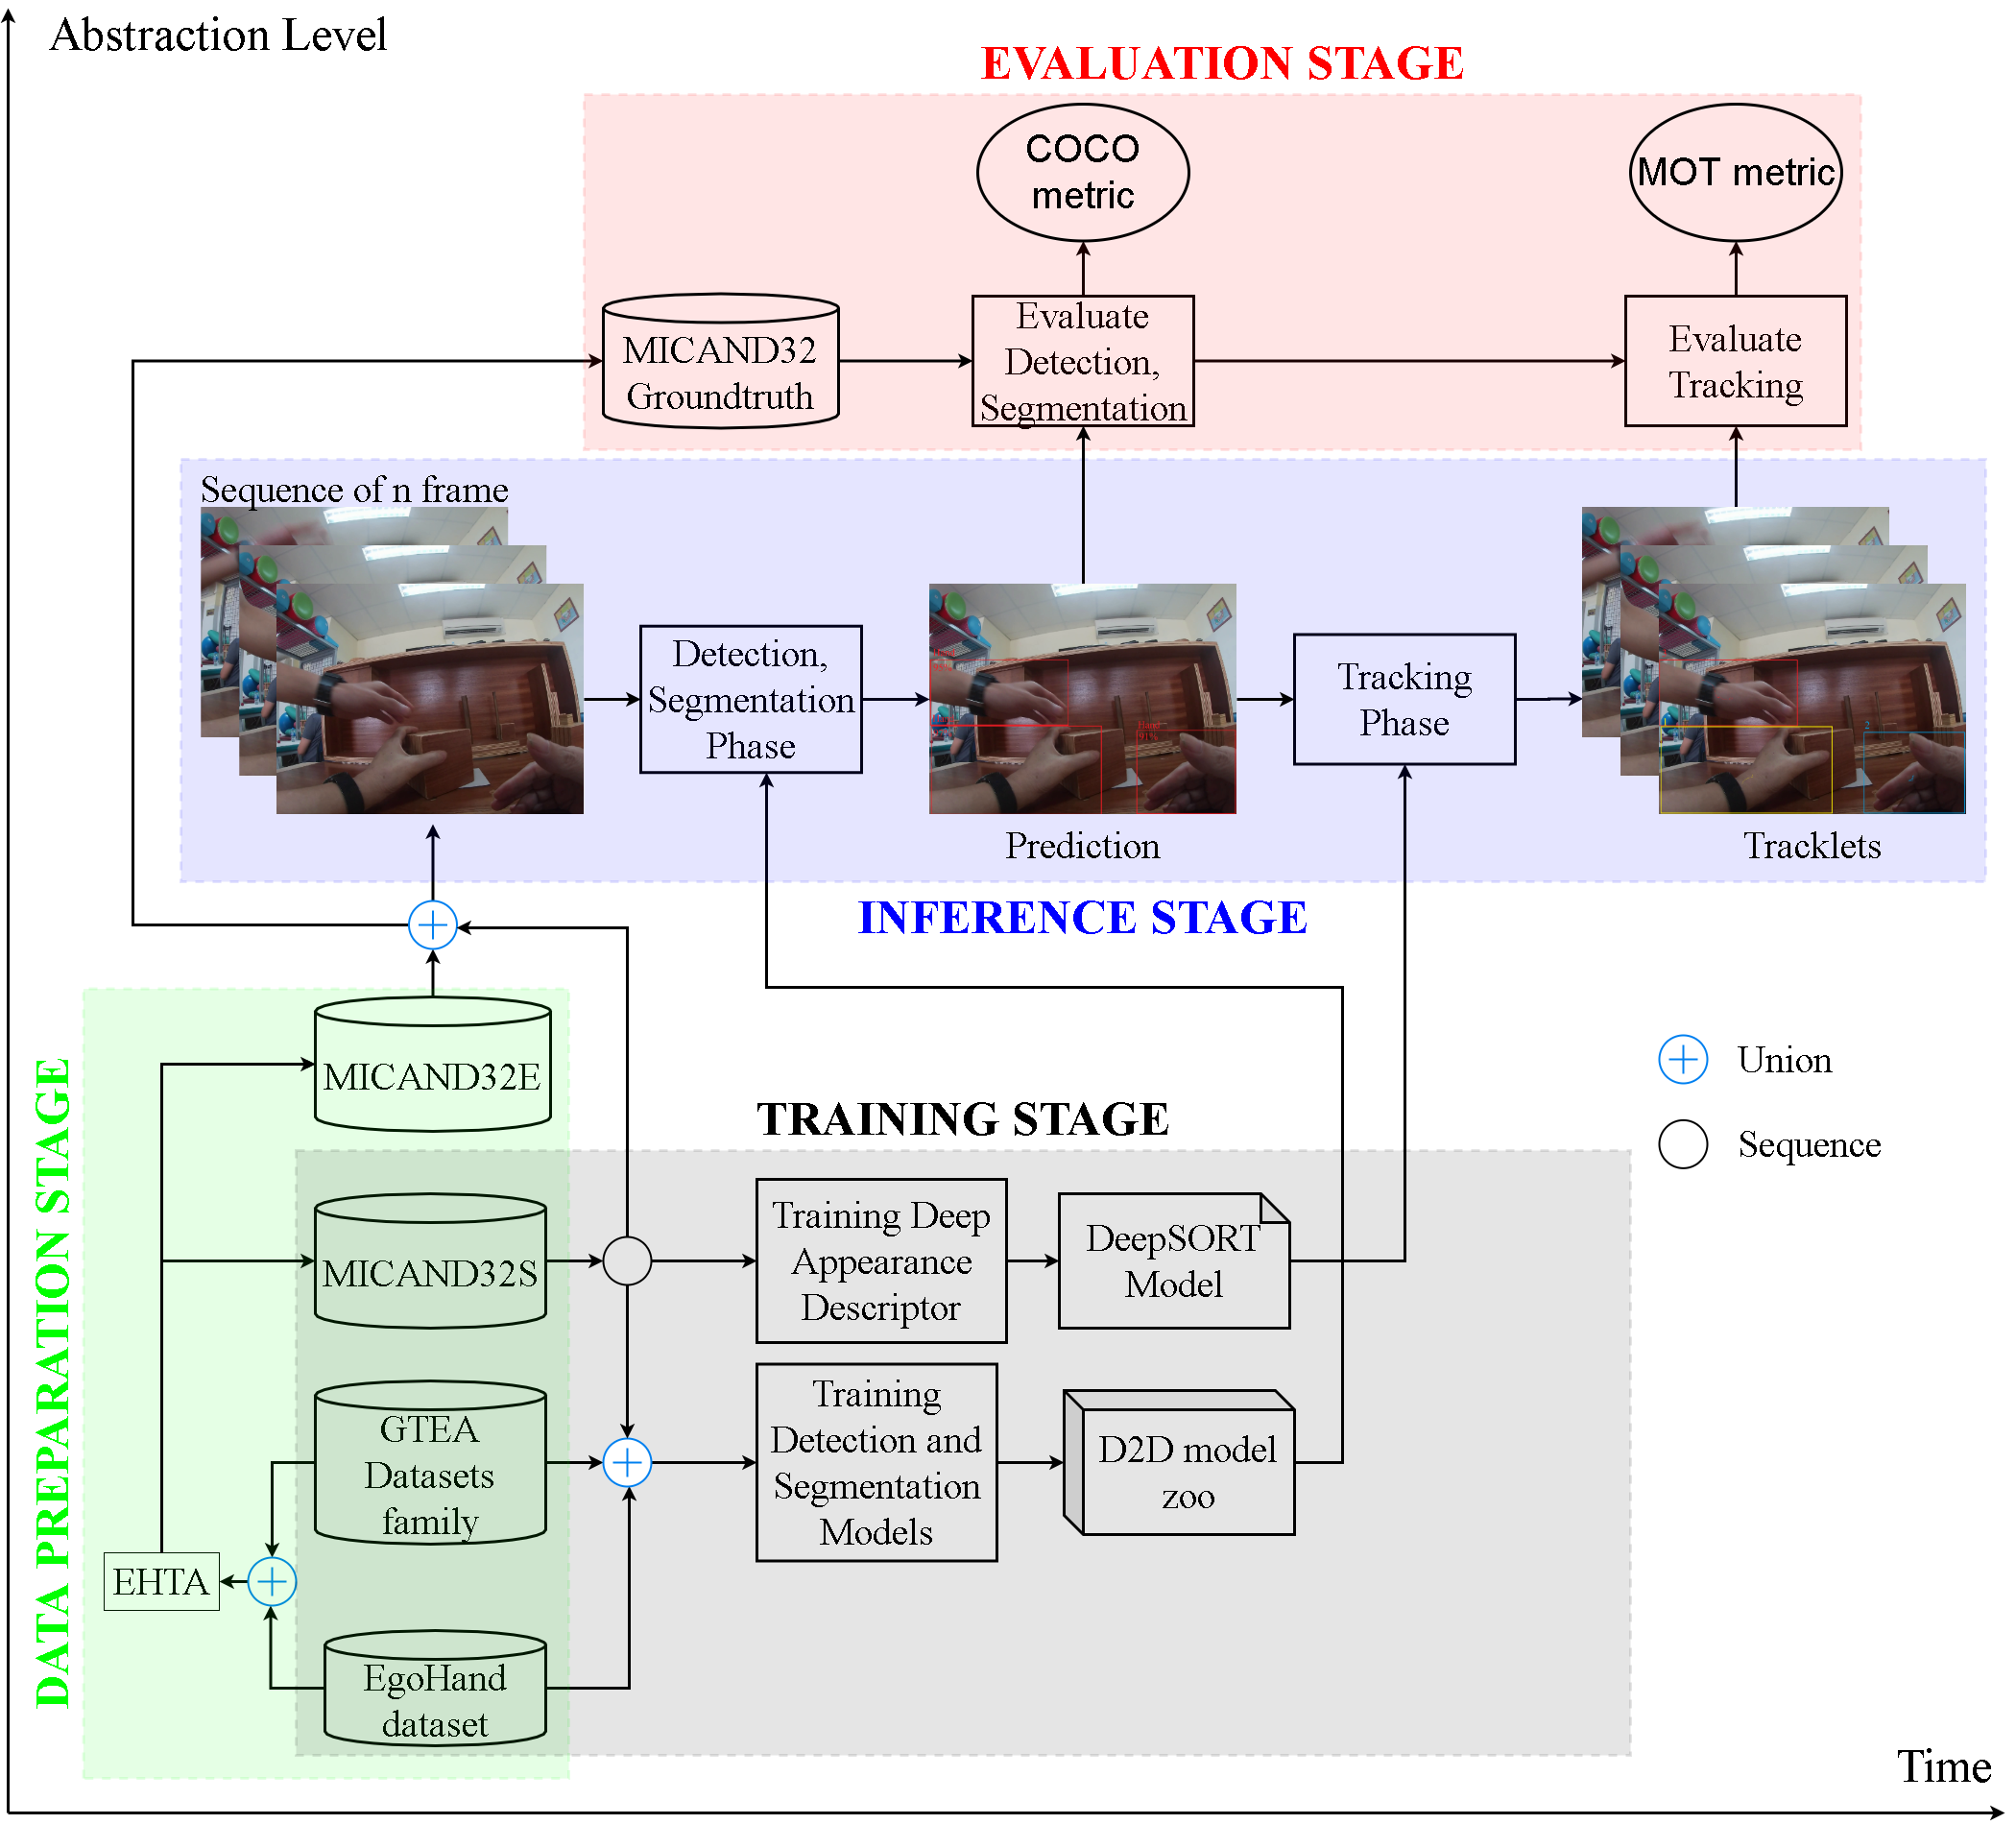
\includegraphics[width=1\linewidth]{Figs/proposedFramework.png}}
	\caption{Overview of proposed framework: D2D. The x-axis represents the time flow of the 4 stages. The y-axis regards the increasing degree of abstraction level of the stages.}
	\label{fig:framework}
\end{figure}
The framework proposed in this thesis consists of 4 stages: \begin{enumerate*}
	\item data preparation stage,
	\item training stage,
	\item inference stage,
	\item evaluation stage
\end{enumerate*}. Initializing with data preparation stage, the GTEA family and EgoHands datasets is collected and is pre-processed in order to keep only suitable and related ground-truth samples. These 2 datasets are used to construct EHTA model zoo by training hand detection and segmentation models from the first-person view. The annotators use semi-automatic EHTA tool to create the new dataset Micand32 descripted in chapter \ref{chap:method}, sub-section \ref{subsec:micand32}. Next is the models training stage. Three datasets including Micand32S, GTEA family and EgoHands datasets is used as fuel to train the hand detection and segmentation from egocentric vision, family of RCNN models and family of YOLO models. At the same time, a deep appearance descriptor is trained on distinct hand groups ground-truth in Micand32S. While the original DeepSORT's descriptor is made in people tracking context, the descriptor trained in the thesis is made well suited for deep metric learning in this egocentric hand context. Detail training techniques are reported in section \ref{sec:trainingstage}. Following the training stage is the inference stage in which all the videos in Micand32 datasets is tested. For each sequence of n frames, each frame in turn is fed respectively into the detection and segmentation phase to get the prediction which locate the hand’s bounding boxes, masks and their confidence scores. This phase requires user to select detection or segmentation algorithm from pre-trained D2D model zoo. Frames with detections are then fed into tracking phase. This phase also requires user to choose tracking algorithm SORT or DeepSORT. The tracking phase indicates the identifications of egocentric hands with their trajectories in the whole video. Section \ref{sec:inferstage} explains in detail the inference procedure. Finally, the evaluation stage encounters. Detection bounding boxes and segmentation masks is be evaluated by comparing with Micand32’s ground-truth. This result is measured in COCO format. The hand’s tracklets is evaluated and reported in MOT Challenge format. Detail evaluation criteria is described in section \ref{sec:evacri}. 
\section{Training stage} \label{sec:trainingstage}
\begin{figure}[htbp]
	\centerline{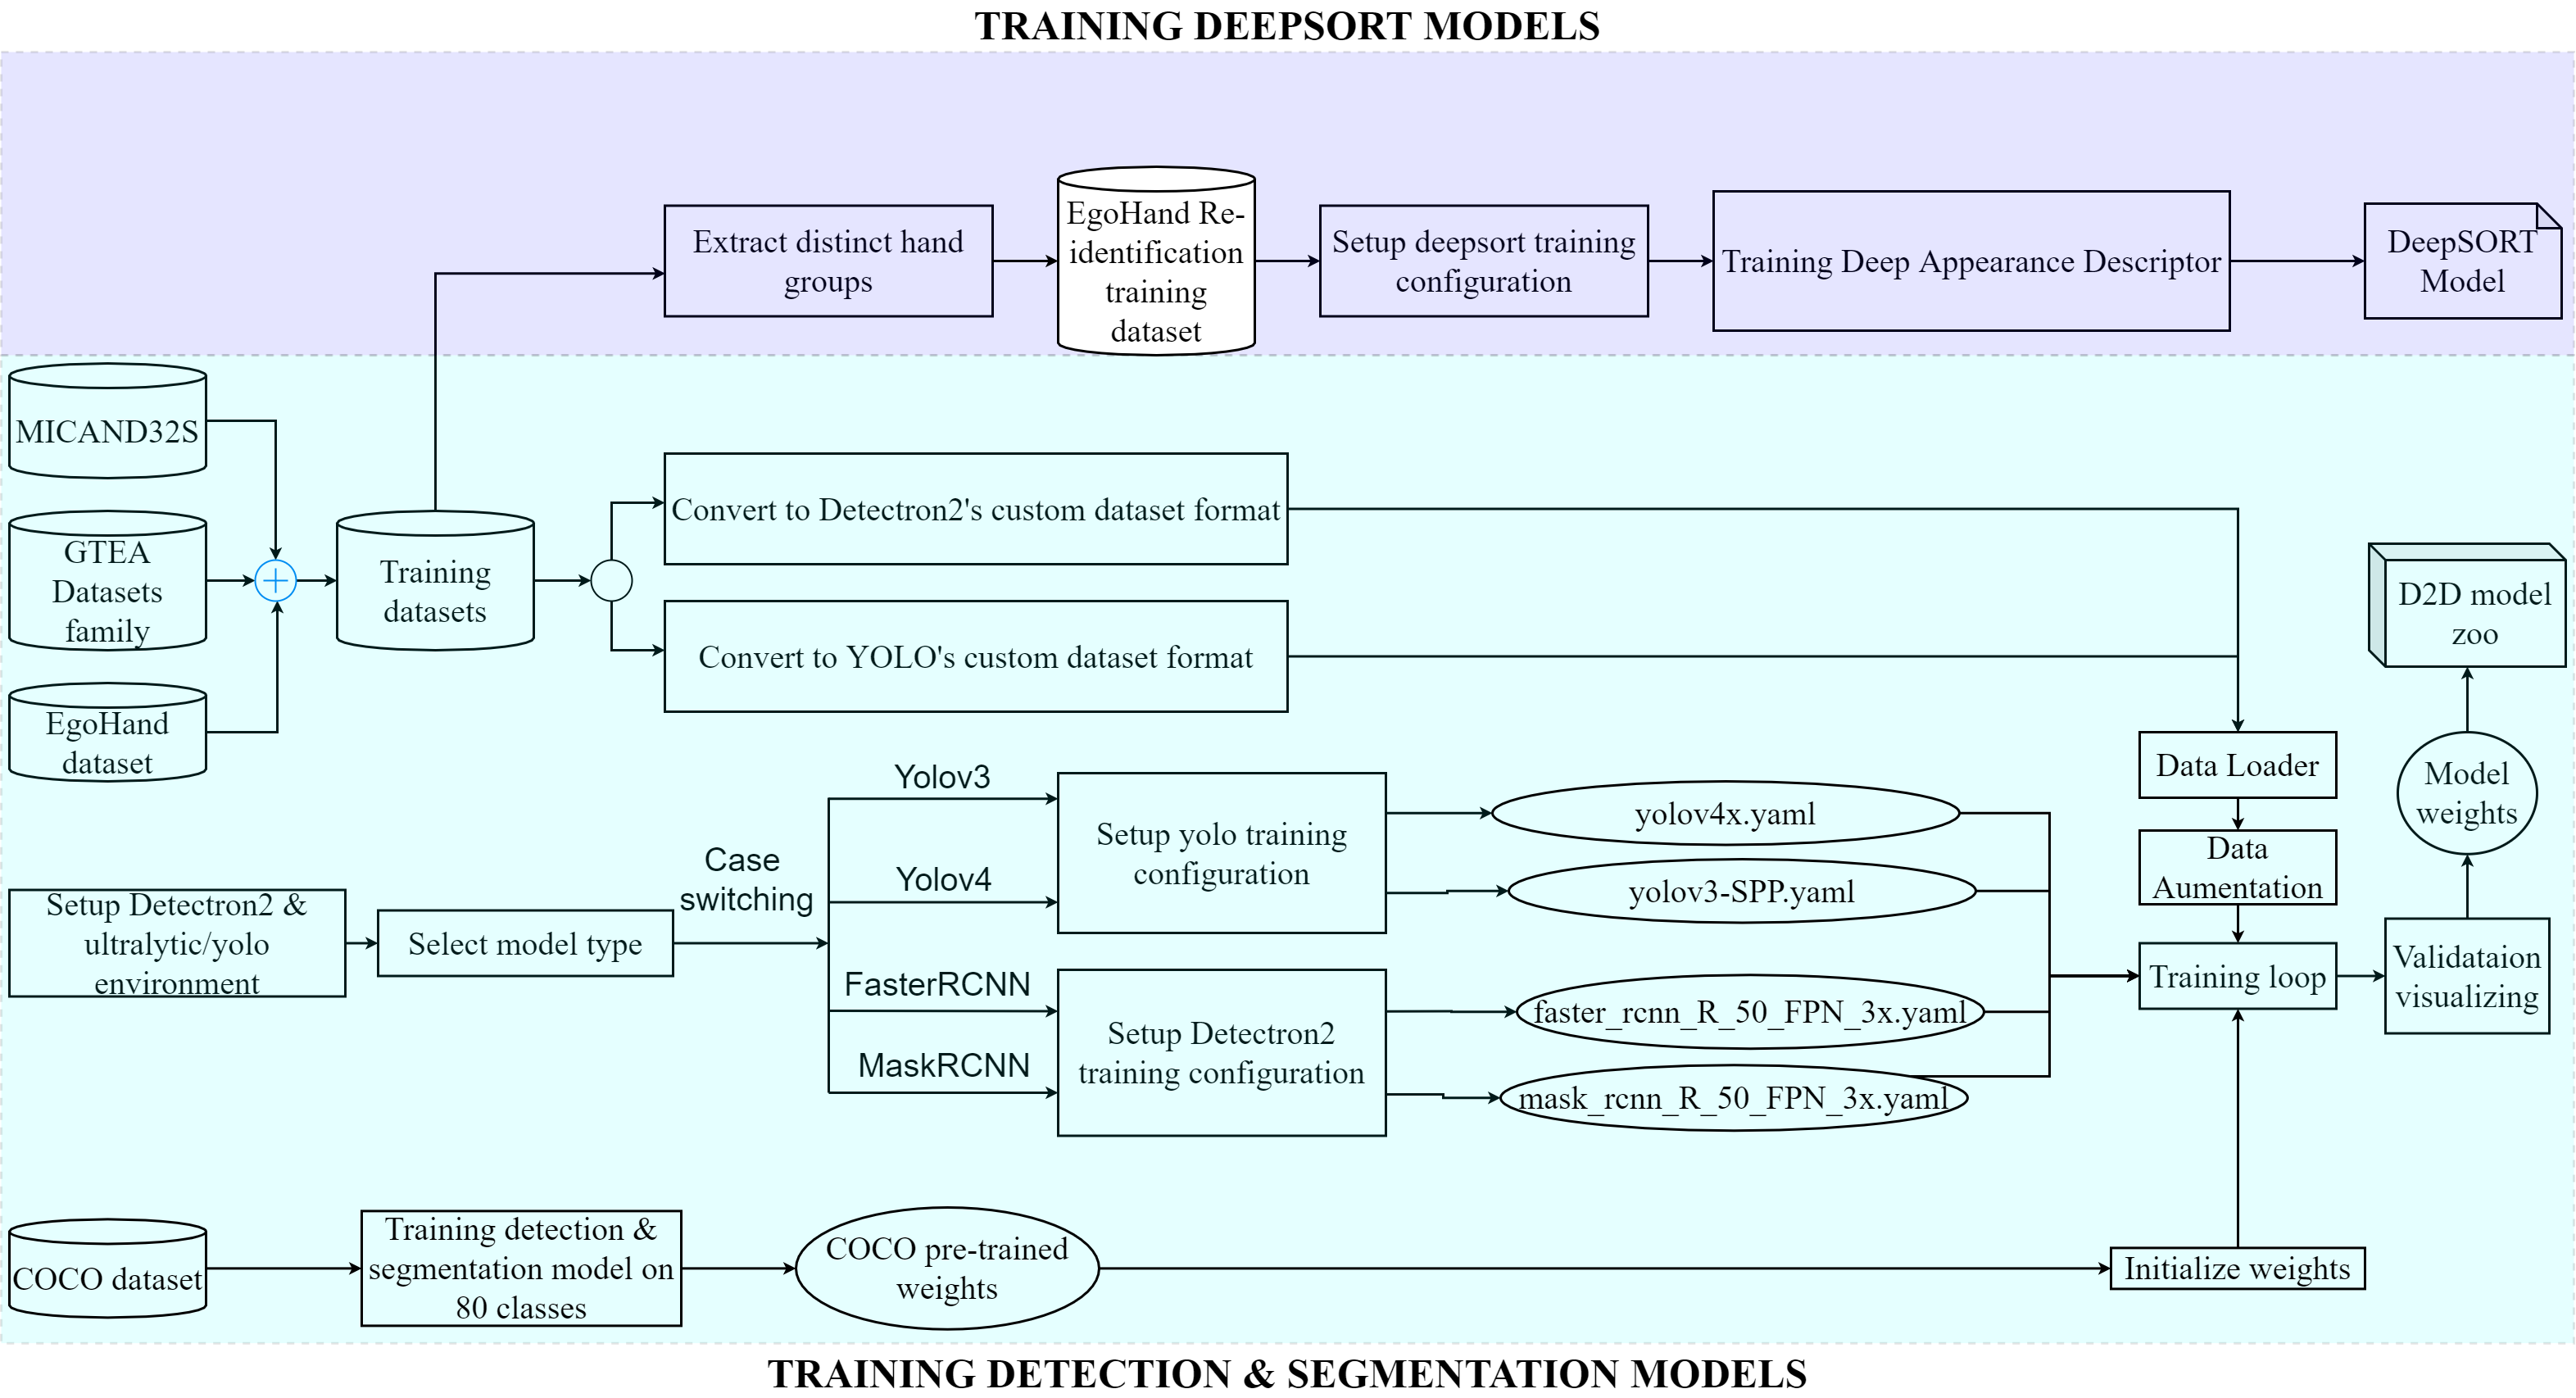
\includegraphics[width=1\linewidth]{Figs/trainingStage.png}}
	\caption{Workflow of the training stage.}
	\label{fig:trainingstage}
\end{figure}
The training stage shown in \ref{fig:trainingstage} consist of parts: \begin{enumerate*}
	\item training detection and segmentation models,
	\item training DeepSORT model
\end{enumerate*}. Input of both parts are the combination of 3 datasets: Miand32S, GTEA family and EgoHands dataset. The first part will generate D2D model zoo which consists 4 types of models, 2 from yolo family and 2 from RCNN family. The second part trains a CNN for deep appearance descriptor for cosine metric learning \cite{DBLP:journals/corr/abs-1812-00442} in DeepSORT. Detail implementation is explained as follow.
\subsection{Training detection and segmentation models}
Initially I setup programming environment which consists 2 frameworks: Detectron2 \cite{wu2019detectron2} for RCNN model family and Ultralytics \cite{ultralytics} for YOLO model family.

Detectron2 is a complete rewrite of the previous version Detectron, and it originates from maskrcnn-benchmark. The platform is now implemented in and powered by the PyTorch deep learning framework. Through a new modular design, Detronron2 is flexible and scalable, and can provide fast training on a single or multiple GPU servers. Detectron2 includes high-quality implementations of state-of-the-art object detection algorithms, including DensePose, panoptic feature pyramid networks, and numerous variants of the pioneering Mask R-CNN model family also developed by FAIR. Its scalable design makes it easy to implement cutting-edge research projects without having to spend the entire code base. The requirements of installing Detectron2 includes: Linux with Python 3.6+, Pytorch 1.4+ and torchvision that matches the PyTorch installation, OpenCV need by demo and visualization. In this thesis, I build Detectron2 from source. The compilers gcc and g++ version 5+ are required, and ninja is recommended for faster build. After having these prerequisites, I clone the Detectron2 repositories and install it via pip from the local clone.

The Ultralytics open-source research into future object detection methods is represented via this repository \cite{ultralytics}. The requirements of install Ultralytics is Python 3.8 or later with all dependencies includes Cython, matplotlib, numpy, OpenCV, pillow, PyYAML, scipy, tensorboard, tqdm, pycocotools, scikit-learn, seaborn, coremltools and onnx. I build Ultralytics from source by cloning their github repository and install via pip.

After installing programming environments, users have to select the model type to train. There are 4 main models integrated in this thesis's framework, the RCNN family consists FasterRCNN and MaskRCNN, while the YOLO family consists Yolov3 and Yolov4. Depending on case of model selection, D2D switches to appropriate branch of setting up training configurations. For the RCNN family, Detectron2 supports different backbone network architectures such as ResNET \{50, 101, 152 \}|, FPN, VGG16, etc. In this thesis, I choose the standard configs, FasterRCNN\_R\_50\_FPN\_3x and MaskRCNN\_R\_50\_FPN\_3x with backbone Resnet 50 layers, feature pyramid network 3x architecture. The config file is saved in a ".h" format file.
\section{Training Deep Appearance Descriptor for DeepSORT}
\section{Inference stage}\label{sec:inferstage}
\begin{figure}[htbp]
	\centerline{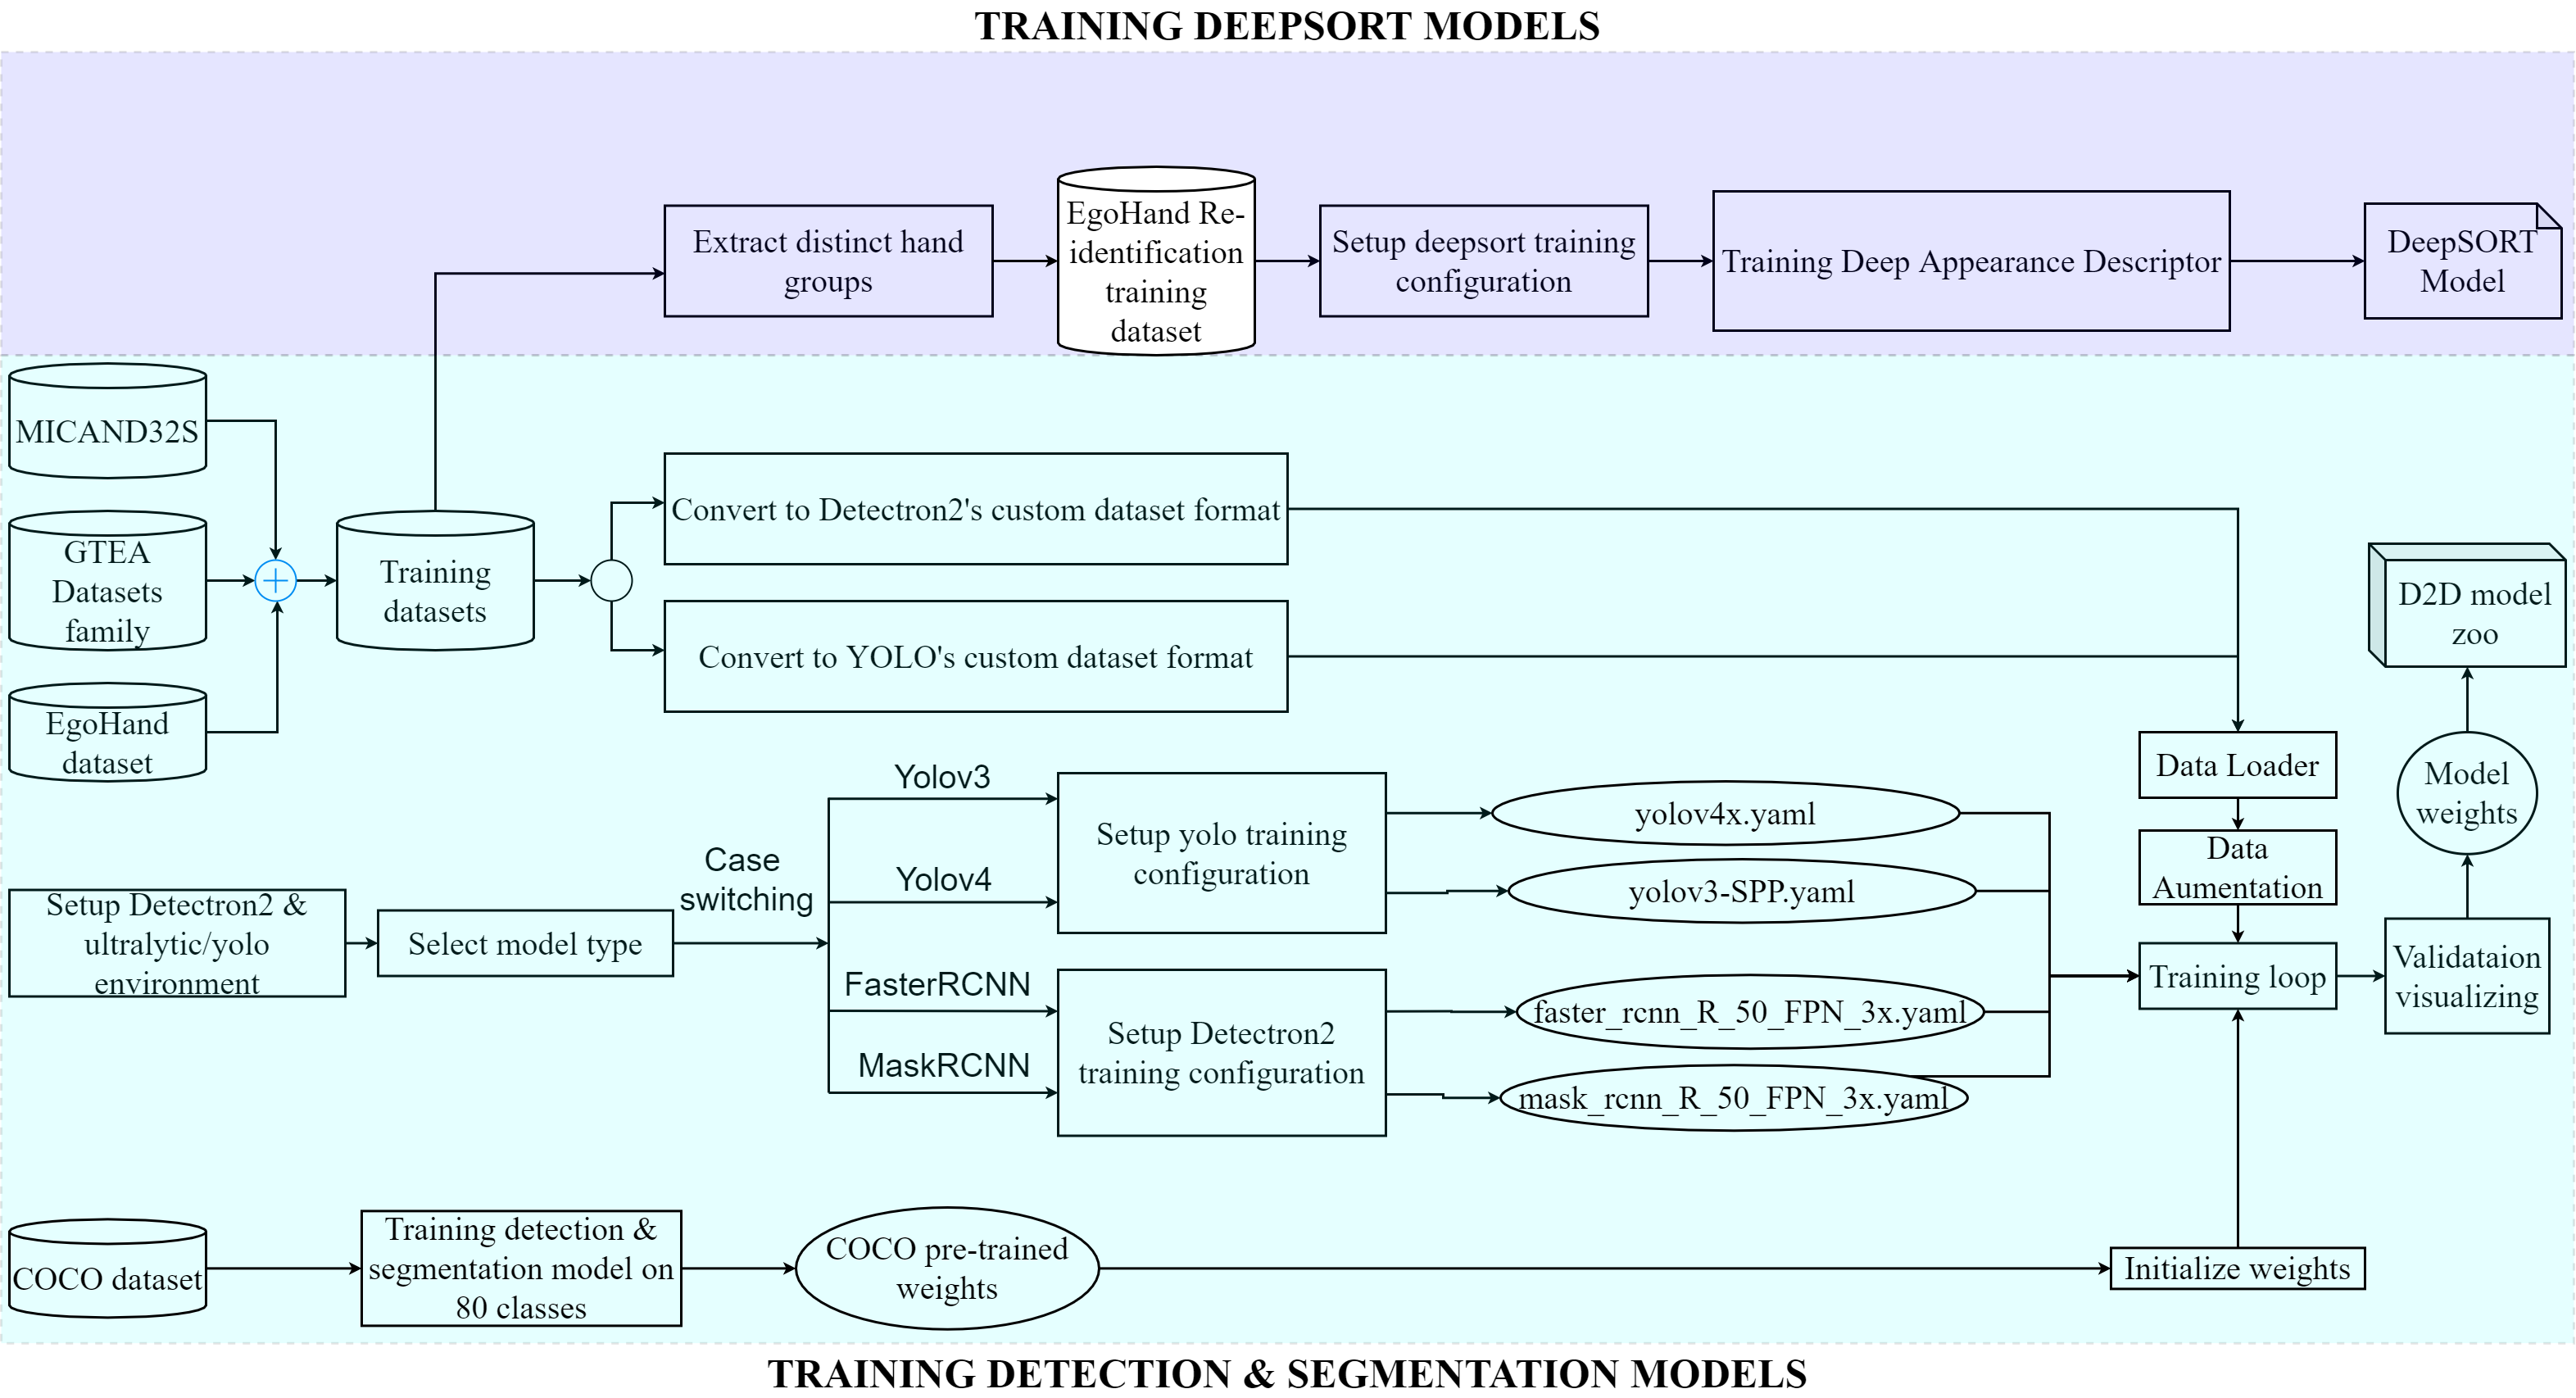
\includegraphics[width=1\linewidth]{Figs/trainingStage.png}}
	\caption{Workflow of inference stage.}
	\label{fig:inferstage}
\end{figure}
\section{Evaluation stage}
Detail evaluation criteria and measurement metrics is reported in chapter \ref{chap:exp}, section \ref{sec:evacri}. The evaluation stage includes 2 parts: (1) evaluate detection and segmentation results; (2) evaluate tracking results. For detection and segmentation result, this thesis adopts the evaluation API from Detectron2 repository and the py-cocotools package. For tracking result, performance is measured according to the framework presented in \cite{DBLP:journals/corr/MilanL0RS16}. The authors provide evaluation scripts for official development kit of MOT Challenge. MOT16 was chosen since it is a compilation of other many metrics developed in an attempt to standardize evaluation of multiple object tracking. This devkit requires Python 3.7+, Matlab R2020a, matlab python engine, pandas and pytz. Tracking result will be saved in simple comma-separated value (CSV) files.